\documentclass[tikz]{standalone}

\usepackage{amsmath} % for \boldsymbol macro
\usepackage{bm}      % for \bm macro
\begin{document}
\begin{tikzpicture}
    \node[anchor=south west,inner sep=0] at (0,0) {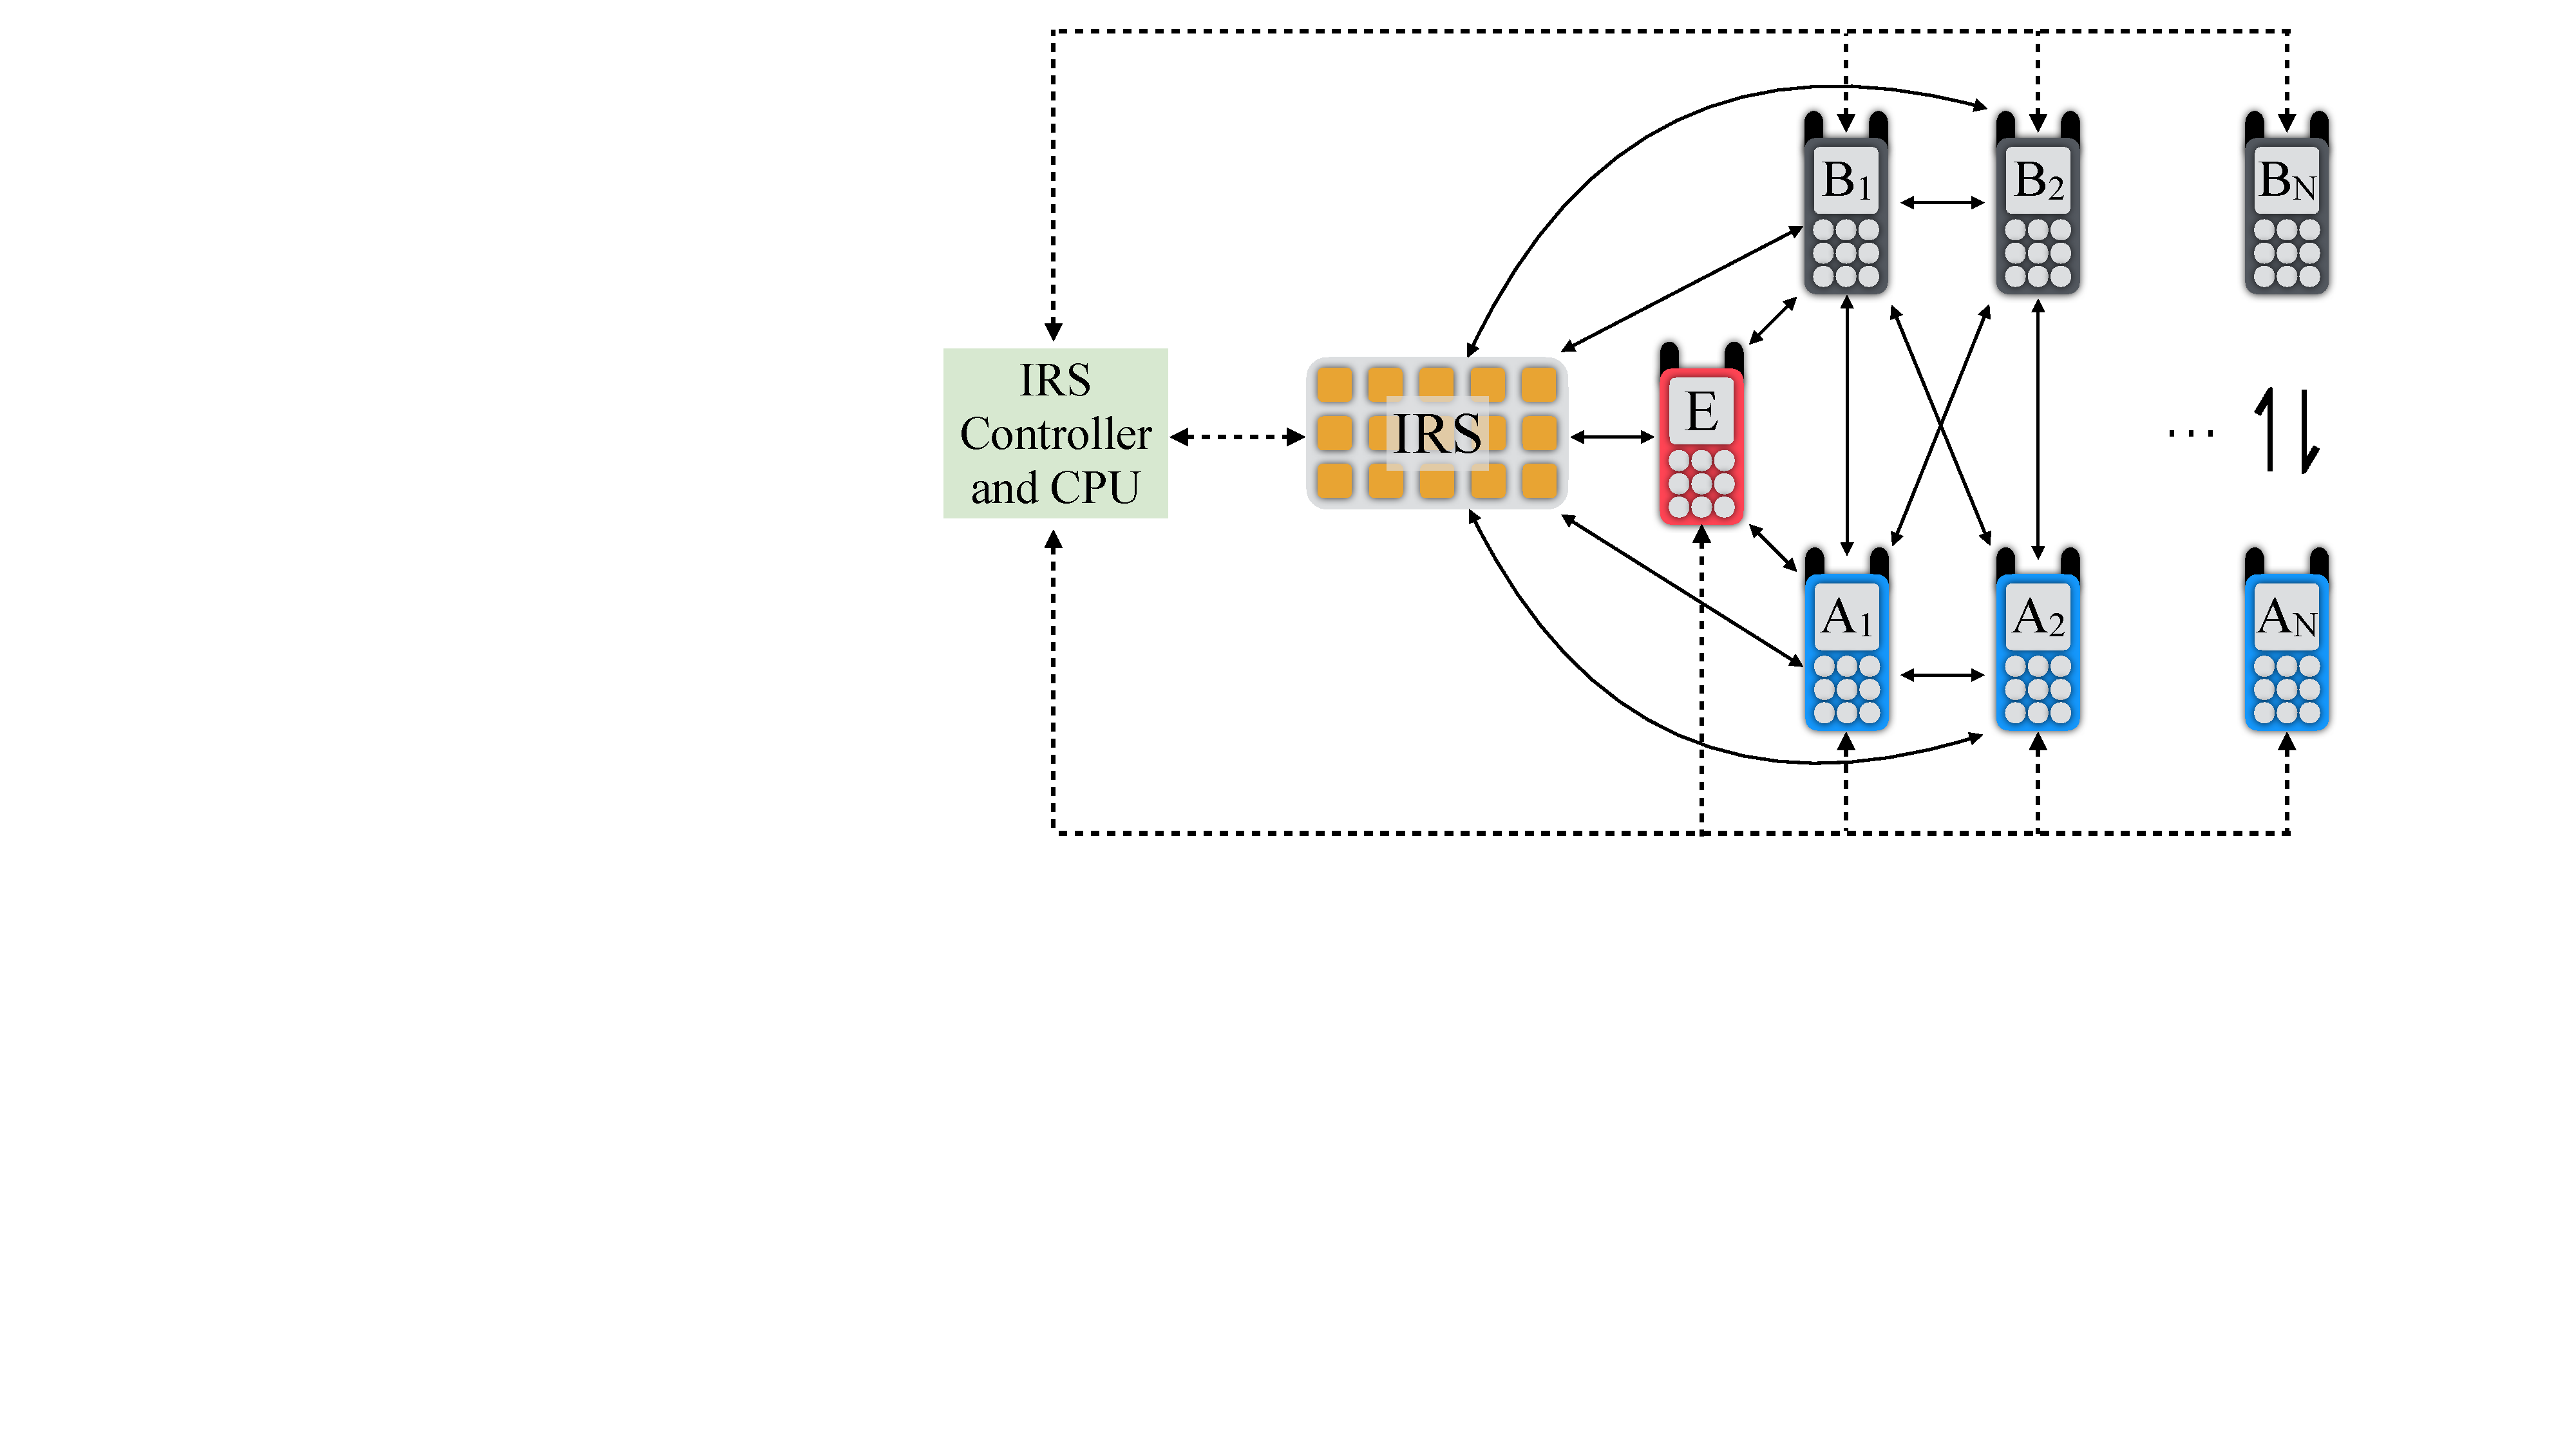
\includegraphics[width=\textwidth]{IRS_design2.pdf}};
    \node[text width=3cm] at (9.32,3.7) {$h_{11}$};
    \node[text width=3cm] at (10.9,3.7) {$h_{22}$};
    \node[text width=3cm] at (10.3,4.15) {$h_{12}$};
    \node[text width=3cm] at (10.3,3.35) {$h_{21}$};    
    
    \node[text width=3cm] at (7.2,2.43) {$\boldsymbol{f}_1$};
    \node[text width=3cm] at (7.2,1.28) {$\boldsymbol{f}_2$};  
    \node[text width=3cm] at (7.2,4.83) {$\boldsymbol{g}_1$};
    \node[text width=3cm] at (7.2,6.23) {$\boldsymbol{g}_2$};
    
    \node[text width=3cm] at (7.2,3.82) {$\boldsymbol{q}$};
    \node[text width=3cm] at (8.57,3) {$q_{A_{1}}$};    
    \node[text width=3cm] at (8.6,4.35) {$q_{B_{1}}$};
    
    \node[text width=3cm] at (9.85,1.95) {$f_{12}$};
    \node[text width=3cm] at (9.85,5.82) {$g_{12}$};
    
\end{tikzpicture}
\end{document}
